\documentclass[aspectratio=169]{beamer}

\usetheme{Madrid}
\usecolortheme{seahorse}

\usepackage[utf8]{inputenc}
\usepackage[T1]{fontenc}
\usepackage{amsmath}
\usepackage{amssymb}
\usepackage{booktabs}
\usepackage{graphicx}
\usepackage{textcomp}
\usepackage{array}

\graphicspath{{figures/}}

\setbeamertemplate{footline}[frame number]
\setbeamertemplate{navigation symbols}{}

\newcommand{\figframe}[3]{% title, file, height fraction
\begin{frame}{#1}
\centering
\includegraphics[width=\textwidth,height=#3\textheight,keepaspectratio]{#2}
\end{frame}}

\title{Hybrid Quantum--Classical Physics-Informed Neural Network \\ for Czochralski Crystal Growth}
\subtitle{Study report --- surrogate training, ibm\_fez hardware inference, and controlled ablation}
\author{Aswin}
\date{October 2026}

\begin{document}

\begin{frame}
\titlepage
\end{frame}

\begin{frame}{Outline}
\tableofcontents
\end{frame}

% =====================================================================
\section{Introduction and Motivation}
% =====================================================================

\begin{frame}{The Industrial Problem}
\begin{itemize}
  \item Czochralski (CZ) crystal growth is the dominant method for producing single-crystal silicon ingots for semiconductor wafers.
  \item A seed crystal is pulled from a molten silicon bath in a rotating quartz crucible at $\sim$1685--1750~K.
  \item Crystal quality (defect density, oxygen concentration, resistivity uniformity) is controlled by melt hydrodynamics and thermal structure.
  \item Modelled with axisymmetric, incompressible Navier--Stokes equations, configured here with:
  \begin{itemize}
    \item $Re = 15$, $Gr = 8{,}000$ (buoyancy), $Pr = 28.463$ (heat transfer)
    \item Rotation-driven swirl
  \end{itemize}
\end{itemize}

\vspace{0.2cm}
\textbf{Five coupled output fields:} $u_r$, $u_z$, $u_\theta$, $p$, $T$

\vspace{0.2cm}
CFD solvers are accurate but slow (hours--days per simulation) --- prohibitive for real-time control or parametric studies.

\vspace{0.1cm}
\scriptsize These dimensionless numbers are the values passed to the training code; they have not been checked against the CFD case set-up (see Appendix, ``Unverified items'').
\end{frame}

\begin{frame}{The Proposed Solution}
\textbf{Hybrid Quantum--Classical Physics-Informed Neural Network (HQPINN)} as a surrogate model:

\begin{itemize}
  \item Takes spatial coordinates $(r, z)$ as input
  \item Produces all five flow fields in milliseconds
  \item Trained on CFD data; Navier--Stokes residuals can be added to the loss
  \item Uses a 16-qubit variational quantum circuit as a feature-extraction layer
  \item Quantum features evaluated on real IBM hardware (inference and noise study); hardware fine-tuning was planned but \textbf{not run}
\end{itemize}

\vspace{0.3cm}
Hypothesis under test: classical expressivity $+$ physics consistency $+$ quantum feature representations improve the surrogate.
\end{frame}

\begin{frame}{Why Quantum Computing?}
\begin{itemize}
  \item Quantum layer: \textbf{96 of 126,021 parameters (0.076\%)}, in parallel with a 64-wide classical skip connection
  \item Motivation: entanglement-based correlations that are hard to reproduce classically
\end{itemize}

\vspace{0.3cm}
\begin{alertblock}{What the measurements say (later sections)}
A controlled ablation (720 runs at 8 qubits, 120 paired comparisons per contrast, plus 12 and 16 qubits) finds \textbf{no benefit from entanglement or from training the quantum weights}, and the quantum branch is measurably worse than a matched classical branch.
\end{alertblock}

This report therefore documents the infrastructure, the real-hardware noise measurements, and the defects found along the way --- not a quantum advantage.
\end{frame}

% =====================================================================
\section{Dataset}
% =====================================================================

\begin{frame}{Dataset Overview}
\textbf{Source:} COMSOL 6.2 axisymmetric simulation of the CZ melt (\texttt{cz\_melt\_raw.txt}).
Domain: $r \in [0, 0.3~\text{m}]$, $z \in [0, 0.15~\text{m}]$.

\vspace{0.3cm}
\begin{table}
\centering
\begin{tabular}{ll}
\toprule
Property & Value \\
\midrule
Total data points & 18,108 \\
Spatial columns & $r$, $z$ \\
Output columns & $u_r$, $u_\theta$ (swirl), $u_z$ (axial), $p$, $T$ \\
Temperature range & 1685--1750~K \\
Pressure range & $-3722$ to $0$~Pa \\
\bottomrule
\end{tabular}
\end{table}

\vspace{0.2cm}
\textbf{Train/Validation split (95/5, seed 42):}
17,203 training points; 905 held out.
\end{frame}

\figframe{CFD fields in physical units}{data_fields}{0.82}

\begin{frame}{Data Normalization}
\begin{table}
\centering
\small
\begin{tabular}{lll}
\toprule
Scale & Value & Derivation \\
\midrule
Length scale & 0.300 m & $\max(r_{max}, z_{max})$ \\
Velocity scale & 0.1666 m/s & max over \emph{all three} velocity components \\
Pressure scale & 3722.41 Pa & max absolute pressure \\
Temp.\ min / max & 1685.0 / 1750.0 K & $\min(T)$, $\max(T)$ \\
Pressure coeff.\ $p_{coeff}$ & 134,128.5 & $p_{scale}/v_{scale}^2$ \\
\bottomrule
\end{tabular}
\end{table}

\begin{alertblock}{Shared velocity scale hides the small components}
The scale is set by the swirl ($|u_\theta|_{max}=0.1666$~m/s). The meridional components peak at only $|u_r|=2.6$ and $|u_z|=1.4$~mm/s, i.e.\ 1.6\% and 0.9\% of that scale, so their normalised MSE ($\sim10^{-6}$) looks excellent while their physical-unit $R^2$ is only 0.87 and 0.84 (Stage 2 results).
\end{alertblock}
\end{frame}

% =====================================================================
\section{Model Architecture}
% =====================================================================

\begin{frame}{Architecture Overview}
\begin{center}
\small
\begin{tabular}{c}
Input $(r, z)$ \\
$\downarrow$ \\
Fourier Feature Encoding $[2 \to 48]$ \\
$\downarrow$ \\
Coordinate Projector $[50 \to 128 \to 128]$ \\
$\downarrow$ \\
ResidualMLP $\times 2$ $[128 \to 128]$ \\
\end{tabular}
\end{center}

\vspace{0.1cm}
\begin{columns}
\column{0.5\textwidth}
\centering
\textbf{to\_quantum} $[128\to64\to16]$, $\pi\cdot\tanh(\cdot)$ \\
$\downarrow$ \\
\textbf{16-Qubit Circuit} (2 layers: RY+RZ+Rot+CZ) \\
$\downarrow$ \\
LayerNorm(16)
\column{0.5\textwidth}
\centering
\textbf{classical\_skip} \\
$[128 \to 64]$, Tanh
\end{columns}

\vspace{0.1cm}
\begin{center}
Concatenate $[64+16+2=82]$ $\to$ Post Network $[82\to128\to64\to5]$ \\
$\to$ Hard constraints in code: output 0 $\times\, r$ and output 2 $\times\, r$
\end{center}
\end{frame}

\begin{frame}{Component Details (1/2)}
\textbf{Fourier Feature Encoding}
\begin{itemize}
  \item Fixed random projection $B \in \mathbb{R}^{2\times24}$, sampled $\mathcal{N}(0, 6^2)$; in the v2 checkpoint $|B|_{max}=19.2$
  \item $\text{ff}(x) = [\sin(2\pi x B), \cos(2\pi x B)]$
\end{itemize}

\vspace{0.2cm}
\textbf{Classical Encoder}
\begin{itemize}
  \item Linear(50, 128) + Tanh, Linear(128, 128) + Tanh
  \item ResidualMLP$\times$2: $h \leftarrow \tanh(h + W_2 \cdot \tanh(W_1 \cdot h))$
\end{itemize}

\vspace{0.2cm}
\textbf{To-Quantum Projection}
\begin{itemize}
  \item Linear(128, 64) + Tanh + Linear(64, 16), scaled by $\pi\cdot\tanh(\cdot)$ to $[-\pi, \pi]$
\end{itemize}
\end{frame}

\begin{frame}{Component Details (2/2)}
\textbf{16-Qubit Variational Quantum Circuit}: RY encoding of the 16 inputs, then 2 layers, each:
\begin{enumerate}
  \item Data re-upload: $RZ(0.5\cdot\theta_{(i+\text{layer}) \bmod 16})$
  \item Trainable rotation: $\text{Rot}(\varphi_i, \theta_i, \omega_i)$ --- 48 params/layer
  \item Entangling: CZ on even pairs, odd pairs, plus a closing CZ (15--0) --- 16 CZ per layer
\end{enumerate}
Measurement: $\langle Z_i \rangle$, $i = 0..15$ \quad $\Rightarrow$ \textbf{96 quantum parameters}

\vspace{0.2cm}
\textbf{Classical skip connection:} Linear(128,64)+Tanh bypasses the quantum layer entirely.

\vspace{0.2cm}
\textbf{Hard constraints (as coded):} output 0 and output 2 are multiplied by $r$, forcing them to vanish on the symmetry axis. In the v2 checkpoint, output 2 was fitted to the \emph{axial} velocity (see ``Defects in the v2 run''), so the constraint sits on the wrong physical field.
\end{frame}

\figframe{Logical quantum circuit (16 qubits, 2 layers)}{circuit_logical}{0.82}

\begin{frame}{Parameter Count}
\begin{table}
\centering
\small
\begin{tabular}{lr}
\toprule
Component & Parameters \\
\midrule
Fourier feature buffer $B$ (frozen) & 48 \\
coord\_proj (2 layers) & 23,040 \\
res1.block (2 layers) & 33,024 \\
res2.block (2 layers) & 33,024 \\
to\_quantum (2 layers) & 9,296 \\
classical\_skip & 8,256 \\
\textbf{q\_layer.weights} & \textbf{96} \\
q\_norm (scale + bias) & 32 \\
post (3 layers) & 19,205 \\
\midrule
\textbf{Total (incl.\ buffer)} & \textbf{126,021} \\
\textbf{Quantum fraction} & \textbf{0.076\%} \\
\bottomrule
\end{tabular}
\end{table}
\end{frame}

% =====================================================================
\section{Physics Loss}
% =====================================================================

\begin{frame}{Governing Equations (as implemented)}
Steady, axisymmetric, incompressible, nondimensionalised; $\rho=1$:

\small
\textbf{Continuity:}
\[ \frac{\partial(r u_r)}{\partial r} + r\frac{\partial u_z}{\partial z} = 0 \]

\textbf{Radial momentum:}
\[ u_r u_{r,r} + u_z u_{r,z} - \frac{u_\theta^2}{r} + p_{coeff}\, p_r - \frac{1}{Re}\Big[u_{r,rr} + \frac{u_{r,r}}{r} - \frac{u_r}{r^2} + u_{r,zz}\Big] = 0 \]

\textbf{Axial momentum:}
\[ u_r u_{z,r} + u_z u_{z,z} + p_{coeff}\, p_z - \frac{1}{Re}\Big[u_{z,rr} + \frac{u_{z,r}}{r} + u_{z,zz}\Big] - \frac{Gr}{Re^2}\theta = 0 \]

where $\theta = (T-T_{min})/(T_{max}-T_{min})$, $Re=15$, $Pr=28.463$, $Gr=8000$, $p_{coeff}=134{,}128$.
\textbf{There is no gravity term $\rho g$}; the buoyancy term acts on $\theta$ only.
\end{frame}

\begin{frame}{Governing Equations (cont.)}
\textbf{Swirl (angular momentum):}
\[ u_r u_{\theta,r} + u_z u_{\theta,z} + \frac{u_r u_\theta}{r} - \frac{1}{Re}\Big[u_{\theta,rr} + \frac{u_{\theta,r}}{r} - \frac{u_\theta}{r^2} + u_{\theta,zz}\Big] = 0 \]

\textbf{Energy:}
\[ u_r \theta_r + u_z \theta_z - \frac{1}{Pr \cdot Re}\Big[\theta_{rr} + \frac{\theta_r}{r} + \theta_{zz}\Big] = 0 \]

\vspace{0.3cm}
\textbf{Implementation:}
\begin{itemize}
  \item All derivatives via \texttt{torch.autograd.grad} with \texttt{create\_graph=True}
  \item \textbf{Quantum detachment:} $q_{out}$ detached in the physics loss --- avoids second-order gradients through the statevector
  \item EMA ($\beta=0.95$) ``balancing'' of the 5 residual terms (found to be a no-op, see defects)
\end{itemize}
\end{frame}

% =====================================================================
\section{Stage 1: Local Proof of Concept}
% =====================================================================

\begin{frame}{Stage 1 --- Mac M4 Pipeline Check}
A quick local run before committing to GPU compute (Mac Mini M4, 24 GB).

\vspace{0.2cm}
\textbf{Configuration:}
\begin{itemize}
  \item 8 qubits, 1 quantum layer; PennyLane \texttt{default.qubit}, \texttt{backprop}, parameter broadcasting
  \item Batch size 2,048, 120 epochs (about 29 minutes, from earlier notes; no log kept)
\end{itemize}

\vspace{0.2cm}
\textbf{What the script does:} data-only loss, OneCycle LR, logs the training loss only.
It has \textbf{no physics loss, no validation split, no per-field logging and no resume}.

\vspace{0.2cm}
\textbf{What it tested:} data loading, normalisation, the quantum layer under broadcasting, checkpoint saving.
\textbf{No validation MSE was measured}, so no accuracy is claimed for this stage.
\end{frame}

% =====================================================================
\section{Stage 2: H100 DGX Pretraining}
% =====================================================================

\begin{frame}{Compute Infrastructure --- Brev H100 DGX}
\begin{table}
\centering
\small
\begin{tabular}{ll}
\toprule
Resource & Specification \\
\midrule
GPU & NVIDIA H100 80GB HBM3 (GPU 4 of 8) \\
Storage & /data volume \\
OS & Ubuntu 22.04 \\
CUDA driver & 580.105.08 (CUDA 13.0) \\
PyTorch & 2.11.0+cu130 \\
PennyLane & 0.44.1 \\
\bottomrule
\end{tabular}
\end{table}

GPUs 0--3 ran a vLLM inference workload; GPU 4 was used for this training.
Launched via \texttt{nohup} with \texttt{CUDA\_VISIBLE\_DEVICES=4}.
\end{frame}

\begin{frame}{Training Configuration}
\begin{table}
\centering
\small
\begin{tabular}{lll}
\toprule
Hyperparameter & Value & Note \\
\midrule
Epochs & 400 & 221.2 min on H100 \\
Batch size & 256 & 68 batches/epoch \\
Learning rate & $2\times10^{-3}$ & CosineAnnealing $\to 10^{-6}$ \\
Physics warmup & epoch 50 & data-only before \\
Physics ramp & \textbf{150 epochs} & linear $0 \to 0.05$, full weight at epoch 200 \\
Physics weight & 0.05 (max) & \\
Grad clip & 1.0 (L2) & \\
EMA beta & 0.95 & ``balancing'' (no-op) \\
Train/val split & 95/5 & 17,203 / 905 \\
Checkpointing & every 50 epochs + best-val & \\
\bottomrule
\end{tabular}
\end{table}
\end{frame}

\begin{frame}{Phase 1: Data-Only Training (Epochs 1--50)}
\begin{table}
\centering
\footnotesize
\begin{tabular}{lllllll}
\toprule
Epoch & Train Loss & Val (sum) & $u_r$ & $u_\theta$ swirl & $u_z$ axial & $p$ / $T$ \\
\midrule
1 & 1.16e-2 & 4.83e-3 & 4.40e-5 & 1.69e-3 & 4.44e-5 & 1.68e-3 / 1.37e-3 \\
10 & 5.92e-5 & 3.11e-4 & 3.61e-6 & 8.57e-5 & 2.46e-6 & 7.24e-5 / 1.47e-4 \\
\textbf{20} & \textbf{5.26e-5} & \textbf{1.58e-4} & \textbf{1.93e-6} & \textbf{5.78e-5} & \textbf{1.44e-6} & \textbf{4.62e-5 / 5.07e-5} \\
30 & 2.96e-5 & 1.75e-4 & 1.20e-6 & 6.51e-5 & 1.12e-6 & 4.58e-5 / 6.15e-5 \\
40 & 4.43e-5 & 3.06e-4 & 2.77e-6 & 1.79e-4 & 9.15e-7 & 6.22e-5 / 6.16e-5 \\
50 & 2.07e-5 & 2.13e-4 & 1.06e-6 & 7.42e-5 & 9.05e-7 & 1.07e-4 / 2.91e-5 \\
\bottomrule
\end{tabular}
\end{table}

\small
``Val (sum)'' is the \emph{sum} of the five per-field normalised MSEs (the mean at epoch 20 is $3.2\times10^{-5}$). Swirl and axial columns are labelled by physical meaning; the log calls them $u_z$ and $u_\theta$ (transposed loader, see defects).

\begin{block}{Best Result}
Best total of $\mathbf{1.58\times10^{-4}}$ at \textbf{epoch 20}, saved as \texttt{pretrained\_v2.best.pt}. Re-evaluating that checkpoint reproduces all five logged per-field values exactly.
\end{block}
\end{frame}

\begin{frame}{Phase 2: Physics Loss Ramp (Epochs 50--200)}
\begin{table}
\centering
\small
\begin{tabular}{lllll}
\toprule
Epoch & Phys.\ Weight & Train Loss & Phys.\ Loss & Val $p$ / $T$ \\
\midrule
60 & 3.33e-3 & 1.01e-1 & 20.05 & 1.05e-1 / 7.53e-2 \\
70 & 6.67e-3 & 6.40e-2 & 4.24 & 1.06e-1 / 7.93e-2 \\
80 & 1.00e-2 & 7.42e-2 & 3.79 & 1.06e-1 / 7.70e-2 \\
100 & 1.67e-2 & 1.50e-1 & 7.19 & 1.06e-1 / 1.05e-1 \\
110 & 2.00e-2 & 2.45e-1 & 11.13 & 2.22e-1 / 1.14e-1 \\
150 & 3.33e-2 & 1.20e-1 & 2.57 & 1.05e-1 / 8.41e-2 \\
200 & 5.00e-2 & 1.09e-1 & 1.37 & 1.06e-1 / 1.02e-1 \\
\bottomrule
\end{tabular}
\end{table}

\begin{alertblock}{Critical Observation}
When the physics loss switched on, validation MSE for $p$ and $T$ jumped from $\sim5\times10^{-5}$ to $\sim0.1$ --- \textbf{three orders of magnitude}. The weight was still only $3\times10^{-3}$.
\end{alertblock}
\end{frame}

\begin{frame}{Phase 3: Full Physics Weight (Epochs 200--400)}
\begin{table}
\centering
\small
\begin{tabular}{llll}
\toprule
Epoch & Train Loss & Physics Loss & Val (sum) \\
\midrule
250 & 8.72e-2 & 9.75e-1 & 0.193 \\
270 & 6.04e-2 & 4.19e-1 & 0.192 \\
\textbf{280} & \textbf{1.04e+9} & \textbf{2.16e+10} & 0.256 \\
\textbf{290} & \textbf{1.18e+14} & \textbf{2.15e+15} & 0.248 \\
300 & 5.57e-2 & 9.62e-2 & 0.246 \\
350 & 5.42e-2 & 4.79e-2 & 0.239 \\
400 & 4.92e-2 & 2.04e-3 & 0.238 \\
\bottomrule
\end{tabular}
\end{table}

At epochs 280--290 the total loss reached $10^9$--$10^{14}$ (cause not diagnosed). Gradient clipping kept the parameters bounded and the loss was back to normal by epoch 300. Final validation stayed at $\sim$0.238, \textbf{1,500$\times$ worse than the best checkpoint}.
\end{frame}

\figframe{Per-field validation MSE through training}{training_val_fields}{0.82}

\begin{frame}{Stage 2 Summary}
\begin{table}
\centering
\begin{tabular}{ll}
\toprule
Metric & Value \\
\midrule
Total wall time & 221.2 minutes (3.69 h) --- from log \\
Time per epoch & $\sim$33 seconds (derived) \\
GPU memory & not recorded \\
\textbf{Best validation (sum of 5 MSEs)} & $\mathbf{1.58\times10^{-4}}$ \textbf{at epoch 20} \\
Final validation & 0.238 at epoch 400 \\
Best checkpoint & \texttt{pretrained\_v2.best.pt} \\
Final checkpoint & \texttt{pretrained\_v2.pt} \\
Export (final weights) & \texttt{pretrained\_v2.ibm.pt} (503 KB) \\
\bottomrule
\end{tabular}
\end{table}
\end{frame}

\figframe{Best checkpoint (epoch 20) vs CFD: $T$ and swirl}{field_maps_best_Tsw}{0.82}
\figframe{Best checkpoint (epoch 20) vs CFD: $u_r$, $u_z$}{field_maps_best_urz}{0.82}

\begin{frame}{Best checkpoint in physical units (all 18,108 nodes)}
\begin{table}
\centering
\small
\begin{tabular}{lrrr}
\toprule
Field & RMSE & Field std & $R^2$ \\
\midrule
$u_r$ & 0.22 mm/s & 0.63 mm/s & 0.875 \\
$u_\theta$ (swirl) & 1.58 mm/s & 17.8 mm/s & 0.992 \\
$u_z$ (axial) & 0.18 mm/s & 0.46 mm/s & 0.841 \\
$p$ & 24.2 Pa & 1221 Pa & 0.9996 \\
$T$ & 0.47 K & 17.7 K & 0.9993 \\
\bottomrule
\end{tabular}
\end{table}

\begin{itemize}
  \item Swirl, $p$ and $T$ are reproduced well; the two meridional velocities are the weak point (shared velocity scale).
  \item Maps cover all nodes, 95\% of which were training points; the logged held-out numbers are on the previous slides.
  \item $p$ is accurate to 24~Pa, but only $0.26$~Pa of $p$ is \emph{not} hydrostatic (next sections): the network is mostly fitting a plane.
\end{itemize}
\end{frame}

% =====================================================================
\section{Stage 3: IBM Quantum Hardware}
% =====================================================================

\begin{frame}{Rationale and What Was Actually Run}
Pretraining used PennyLane's noiseless \texttt{default.qubit}. On real hardware the quantum features $\langle Z_i\rangle$ are perturbed by gate and readout errors, and the classical head was only ever trained on clean features.

\vspace{0.2cm}
\textbf{Planned:} freeze the circuit and fine-tune the classical head on hardware outputs.

\vspace{0.2cm}
\textbf{Actually run:} \emph{inference only.} Before its training loop the script evaluates the model on 2,000 random points (seed 42) for a ``predictions vs ground truth'' plot; on a remote device each point is one hardware job. All 818 jobs were these evaluations.

\vspace{0.2cm}
\begin{alertblock}{Fine-tuning never started}
\texttt{ibm\_train.log} has no training lines, no fine-tuned checkpoint was written, and the plan time ran out first. Fine-tuning is \textbf{planned work}.
\end{alertblock}
\end{frame}

\begin{frame}{IBM Quantum Backend}
\begin{table}
\centering
\small
\begin{tabular}{ll}
\toprule
Property & Value \\
\midrule
Backend & \textbf{ibm\_fez}, 156-qubit \textbf{Heron r2} \\
Calibration (24 Apr 2026, 18:54 CEST) & median CZ error $2.6\times10^{-3}$ \\
 & median SX error $2.8\times10^{-4}$ \\
 & median readout error $1.5\times10^{-2}$ \\
Transpilation & optimisation level 1 \\
Error mitigation & measurement twirling + measurement mitigation (TREX) \\
Dynamical decoupling & disabled \\
Shots per job & 4,096 (precision $1/64$) \\
Instance & hybrid\_qcpinn (flex plan) \\
\bottomrule
\end{tabular}
\end{table}
\end{frame}

\begin{frame}{The Hardware Session}
\begin{table}
\centering
\small
\begin{tabular}{ll}
\toprule
Metric & Value \\
\midrule
Window & 24 Apr 20:07 -- 25 Apr 01:23 (UTC+2), 5.3 h \\
Jobs submitted & \textbf{818} (815 DONE, 3 cancelled) \\
QPU time (billed, DONE jobs) & 9,826 s (2.7 h), $\approx$12 s per job \\
Mean submission rate & 2.6 jobs/min; 46\% of gaps $<$ 5 s \\
Distinct points evaluated & \textbf{303} of the 2,000 planned \\
Points run more than once & 267 (up to 3 copies) \\
\bottomrule
\end{tabular}
\end{table}

\small
The repeats and the short gaps are consistent with two to three copies of the script running at once with the same seed (same points, same order). Plan time ran out at 01:23 (\texttt{ibm\_train.log}). Earlier versions of this deck said 500 jobs because the job listing was capped at 500; all 818 were retrieved on 1 Oct 2026.
\end{frame}

\begin{frame}{Transpiled Circuit on ibm\_fez}
\begin{columns}
\column{0.5\textwidth}
\textbf{Logical circuit:}
\begin{itemize}
  \item 16 RY, 32 RZ, 32 Rot, \textbf{32 CZ}
\end{itemize}
\textbf{After transpilation (bound circuits, from the jobs):}
\begin{itemize}
  \item CZ: 50--104 (median 83)
  \item SX: 96--196 (median 156)
  \item RZ: 96
  \item Depth: 30--90
  \item 16--23 physical qubits active (routing SWAPs)
\end{itemize}
\column{0.5\textwidth}
\centering
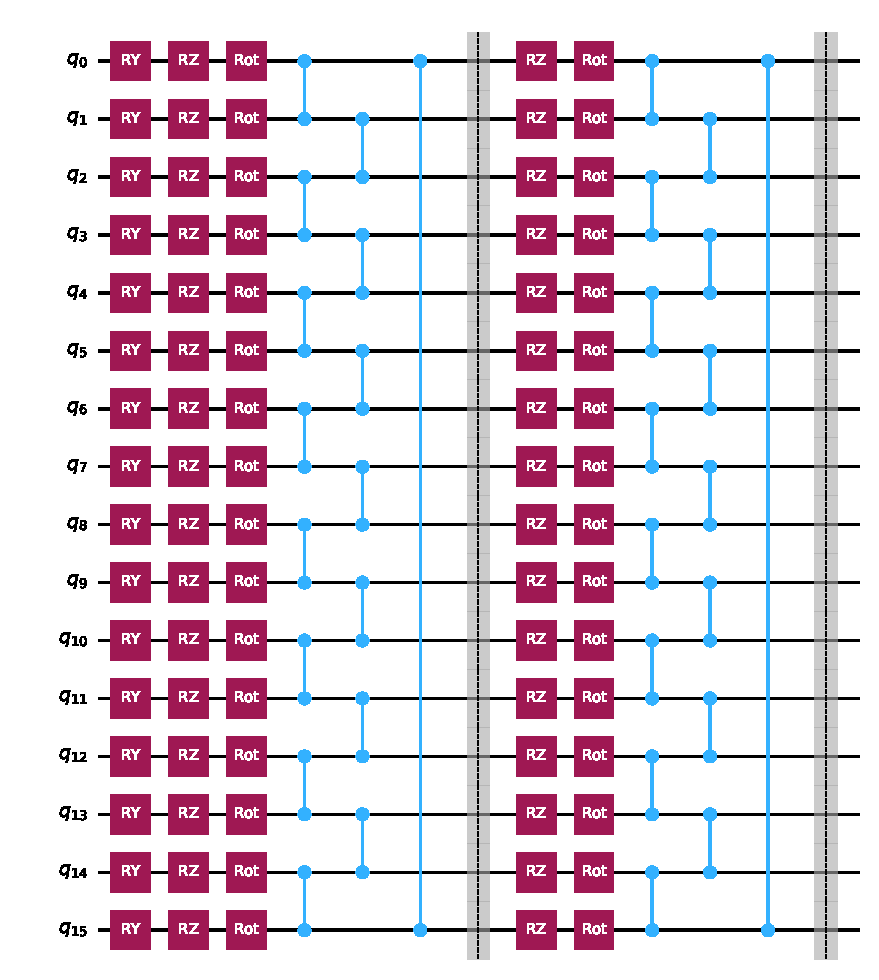
\includegraphics[width=\textwidth,height=0.7\textheight,keepaspectratio]{circuit_logical}
\end{columns}

\vspace{0.1cm}
\small This replaces the earlier ``$\sim$50 gates per shot'' estimate.
\end{frame}

\figframe{Hardware vs noiseless $\langle Z_i\rangle$ (815 jobs $\times$ 16 qubits)}{ibm_hw_vs_sim}{0.62}

\begin{frame}{Hardware vs Noiseless: Numbers}
Noiseless reference: exact simulation of each job's own bound, transpiled circuit.

\begin{itemize}
  \item Mean $|\text{hardware} - \text{noiseless}| = 0.038$ (RMSE 0.050), correlation 0.9966
  \item Hardware values are shrunk toward zero: fitted slope \textbf{0.94}
  \item Shot noise is only $\sigma\approx0.014$; just 64\% of deviations fall within $3\sigma$ --- the rest is systematic hardware error
  \item Per-qubit bias reaches $+0.06$ (qubits 13, 14), $-0.03$ (qubits 1, 7)
  \item Repeats of the same point differ by 0.030 on average (std), about twice shot noise: run-to-run drift
\end{itemize}

\vspace{0.2cm}
\begin{block}{Validation of the mapping}
Every one of the 815 jobs matches \texttt{pretrained\_v2.best.pt}'s noiseless features to $\sim10^{-14}$; no other checkpoint matches. So all hardware jobs used the epoch-20 best checkpoint and the first 303 distinct points of the seed-42 sample.
\end{block}
\end{frame}

\figframe{Effect on predictions: classical head fed hardware features}{ibm_head_with_hardware}{0.62}

\begin{frame}{Effect on Predictions}
Classical head and weights unchanged (no fine-tuning); only the 16 quantum features replaced by hardware values.

\begin{table}
\centering
\small
\begin{tabular}{lrr}
\toprule
RMSE & noiseless features & ibm\_fez features \\
\midrule
$T$ & 0.40 K & 0.97 K \\
$p$ & 22 Pa & 37 Pa \\
$u_\theta$ (swirl) & 2.3 mm/s & 3.3 mm/s \\
Mean of 5 normalised MSEs & $5.2\times10^{-5}$ & $1.4\times10^{-4}$ \\
\bottomrule
\end{tabular}
\end{table}

\begin{itemize}
  \item Hardware noise raises the mean MSE \textbf{2.7$\times$}; $T$ is hit hardest (6.0$\times$).
  \item This is the one result the IBM time produced. 303 points, mostly training points; it measures noise sensitivity, not generalisation.
  \item Recovering this loss is what the planned head fine-tuning would target.
\end{itemize}
\end{frame}

\figframe{Job submission timeline (corrected)}{ibm_job_timeline}{0.62}

\begin{frame}{Status of the IBM Work}
\begin{itemize}
  \item \textbf{Done:} 815 hardware inference jobs, exact noiseless comparison, effect on predictions, real transpiled-circuit statistics, calibration snapshot.
  \item \textbf{Not done:} head fine-tuning on hardware (the planned Stage 3); no hardware-trained checkpoint exists.
  \item No QPU plan time remains. Job records and results were retrieved read-only on 1 Oct 2026 (the saved key still authenticated) and stored in \texttt{ibm\_results/}.
  \item If hardware is available again: run the training loop \emph{without} the 2,000-point diagnostic, and with one process only.
\end{itemize}
\end{frame}

% =====================================================================
\section{Weight Diagnostics}
% =====================================================================

\begin{frame}{Quantum Circuit Weights (best checkpoint, epoch 20)}
\begin{columns}
\column{0.42\textwidth}
\small
\begin{tabular}{ll}
\toprule
Statistic & Value \\
\midrule
Shape & (2, 16, 3) \\
Mean & 3.492 rad \\
Std & 1.788 rad \\
Min & 0.003 rad \\
Max & 6.272 rad \\
\bottomrule
\end{tabular}

\vspace{0.2cm}
\small Angles spread over $[0, 2\pi]$; none stuck at 0 or $\pi$. With $\sim$0.08\% of the parameters this says little about whether they matter --- the ablation says they do not.
\column{0.58\textwidth}
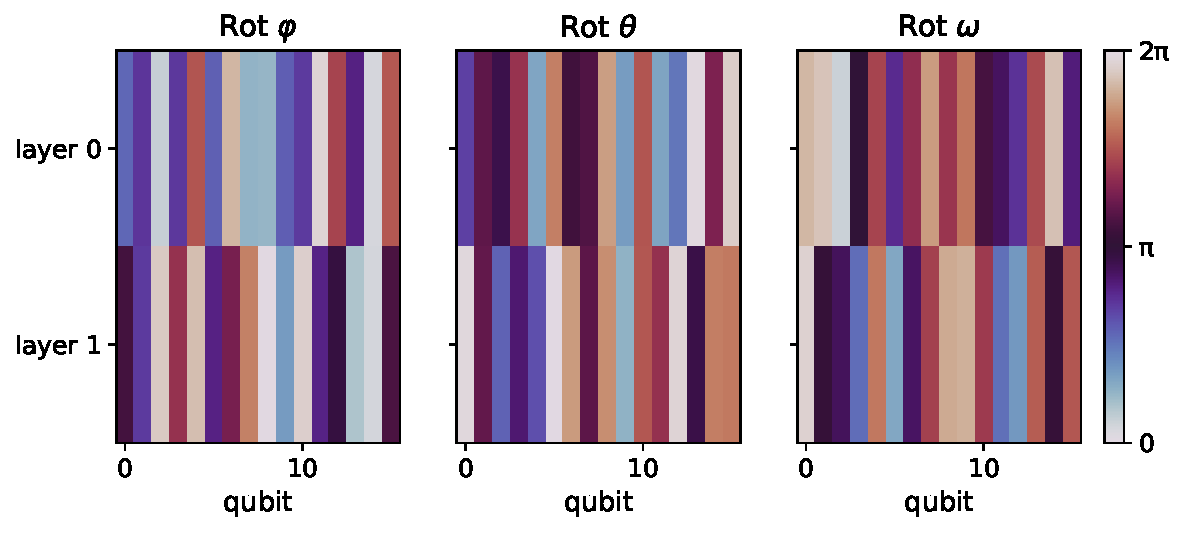
\includegraphics[width=\textwidth]{quantum_weights_heatmap}
\end{columns}
\end{frame}

\begin{frame}{Quantum LayerNorm (best checkpoint)}
\begin{table}
\centering
\begin{tabular}{lll}
\toprule
Statistic & Scale $\gamma$ & Bias $\beta$ \\
\midrule
Min & 0.938 & $-0.035$ \\
Max & 1.002 & $+0.023$ \\
Mean & 0.981 & $-0.0005$ \\
\bottomrule
\end{tabular}
\end{table}

\begin{alertblock}{Interpretation}
$\gamma\approx1$ and $\beta\approx0$: at epoch 20 the LayerNorm has barely moved from its initialisation, so all 16 qubit features are weighted nearly equally.
\end{alertblock}
\end{frame}

\begin{frame}{Classical Weight Distributions (best checkpoint)}
\begin{table}
\centering
\scriptsize
\begin{tabular}{lrrr}
\toprule
Layer & Mean & Std & Max $|w|$ \\
\midrule
ff.B (Fourier, frozen) & $-0.832$ & 6.282 & 19.20 \\
coord\_proj.0 & $-0.001$ & 0.083 & 0.263 \\
coord\_proj.2 & 0.001 & 0.057 & 0.186 \\
res1.block.0 / .2 & 0.000 / 0.001 & 0.054 / 0.053 & 0.142 / 0.148 \\
res2.block.0 / .2 & 0.000 / 0.000 & 0.053 / 0.052 & 0.138 / 0.174 \\
to\_quantum.0 / .2 & $-0.001$ / 0.001 & 0.053 / 0.073 & 0.146 / 0.184 \\
classical\_skip.0 & $-0.001$ & 0.052 & 0.133 \\
post.0 / .2 / .4 & 0.000 / 0.001 / 0.002 & 0.065 / 0.053 / 0.067 & 0.229 / 0.141 / 0.140 \\
\bottomrule
\end{tabular}
\end{table}
All classical layers are zero-mean with small weights (std 0.05--0.08). Earlier versions of this slide mixed in values from the older v1 checkpoint (std 0.17--0.36).
\end{frame}

\begin{frame}{Output Layer and Fourier Frequencies}
\textbf{Output layer (post.4)} maps 64 hidden units $\to$ 5 channels:
\begin{itemize}
  \item Mean $|w|$ per channel is 0.053--0.062: \textbf{no channel dominates}
  \item Output biases: $-0.10$, $-0.05$, $+0.03$, $-0.11$, $-0.11$ (the earlier ``$T$ bias $+0.22$'' came from v1)
\end{itemize}

\vspace{0.3cm}
\textbf{Fourier matrix $B$} (frozen at initialisation):
\begin{itemize}
  \item Entries span about $\pm19$ (std 6.3, consistent with $\mathcal{N}(0,6^2)$)
  \item The largest entry (19.2) is in the $z$ row, column 0
\end{itemize}
\end{frame}

% =====================================================================
\section{Why Physics Loss Failed}
% =====================================================================

\begin{frame}{Quantitative Impact}
\begin{table}
\centering
\small
\begin{tabular}{lllr}
\toprule
Field & Best (ep.\ 20) & Final (ep.\ 400) & Degradation \\
\midrule
$u_r$ & $1.93\times10^{-6}$ & $1.79\times10^{-4}$ & \textbf{93$\times$} \\
$u_\theta$ (swirl) & $5.78\times10^{-5}$ & $8.83\times10^{-3}$ & \textbf{153$\times$} \\
$u_z$ (axial) & $1.44\times10^{-6}$ & $5.06\times10^{-5}$ & \textbf{35$\times$} \\
\textbf{$p$} & $\mathbf{4.62\times10^{-5}}$ & $\mathbf{0.100}$ & \textbf{2,165$\times$} \\
\textbf{$T$} & $\mathbf{5.07\times10^{-5}}$ & $\mathbf{0.129}$ & \textbf{2,544$\times$} \\
\bottomrule
\end{tabular}
\end{table}

\small
Normalised validation MSE. The variance of normalised $p$ is 0.108 and of $T$ is 0.074: the final $p$ error (0.100) is that of a \textbf{flat prediction}, and the final $T$ error (0.129) is \textbf{worse than predicting the mean}.
\end{frame}

\figframe{Per-field degradation, best vs final}{physics_impact}{0.8}

\figframe{The CFD pressure is purely hydrostatic}{pressure_hydrostatic}{0.72}

\begin{frame}{Root Cause: What the Physics Loss Asked For}
\begin{itemize}
  \item CFD $p$ is hydrostatic: a linear fit in $z$ gives slope $-24{,}811$~Pa/m, i.e.\ $\rho=2{,}529$~kg/m$^3$ (liquid-silicon scale), $1-R^2=4\times10^{-8}$.
  \item After removing it only \textbf{0.26 Pa} of variation remains, out of 3,722~Pa. ``Predicting $p$'' is fitting a plane.
  \item The implemented $z$-momentum has \textbf{no $\rho g$ term and $\rho=1$}. For the CFD pressure the pressure-gradient term alone is $p_{coeff}\,\partial\hat p/\partial\hat z=-2.7\times10^{5}$, balanced by nothing. \textbf{The CFD solution itself violates this residual by $\approx2.7\times10^{5}$.}
  \item Reducing that residual means flattening $p$; the network's final $p$ is flat (MSE 0.100 vs variance 0.108).
\end{itemize}

\vspace{0.2cm}
\begin{alertblock}{Withdrawn}
The earlier explanation (``$p_{coeff}$ vs $1/Re$, a 2,000,000:1 imbalance'') and its fix (weight $p$ by $1/p_{coeff}^2$) are retracted: re-weighting cannot make an inconsistent equation consistent.
\end{alertblock}
\end{frame}

\begin{frame}{Defects in the v2 Run (\texttt{DEFECTS-2026-08.md})}
Found in August on MeLuXina CPU nodes; fixes were applied to the mainline scripts \emph{after} the v2 checkpoint was trained.

\begin{enumerate}
  \item \textbf{Transposed velocity columns.} The loader put the swirl column in the axial slot and vice versa. In the log, ``$u_z$'' is swirl and ``$u_\theta$'' is axial; the physics residual was applied to the swapped fields too.
  \item \textbf{One shared velocity scale}, which suppresses $u_r$ and $u_z$ by 64$\times$ and 115$\times$ in normalised space.
  \item \textbf{EMA ``balancing'' is a no-op:} the physics term entered at 20 against a data loss of $2\times10^{-5}$ --- six orders of magnitude --- and validation went from $2\times10^{-4}$ to 0.24.
\end{enumerate}

\vspace{0.2cm}
Reported in that document (not re-run here): with the fixes and magnitude-normalised balancing the physics-on fit reaches the data-only ceiling. Combined with the hydrostatic finding, this means the physics term then barely constrains $p$.
\end{frame}

\begin{frame}[fragile]{Loss Explosion at Epoch 280}
\begin{verbatim}
[0280/400] loss=1.0368e+09 data=5.0592e-02 phys=2.1591e+10
[0290/400] loss=1.1795e+14 data=4.9662e-02 phys=2.1481e+15
[0300/400] loss=5.5708e-02 data=4.8543e-02 phys=9.6150e-02
\end{verbatim}

\vspace{0.3cm}
\begin{itemize}
  \item Data loss stayed $\sim$0.05; the explosion is entirely in the physics residual
  \item Gradient clipping (max norm 1.0) bounded the update; recovered by epoch 300
  \item Cause not diagnosed (the earlier boundary-condition explanation was a guess)
\end{itemize}
\end{frame}

\begin{frame}{Recommended Fix}
\begin{alertblock}{Rebuild the physics loss before re-weighting it}
\begin{enumerate}
  \item Use the \textbf{reduced pressure} $p+\rho g z$ with $\rho=2{,}529$~kg/m$^3$ and the real density in the momentum equations.
  \item Check $Re$, $Pr$, $Gr$ against the CFD case ($Pr=28.463$ is far from liquid silicon, $\sim$0.01).
  \item Add boundary-condition terms.
  \item Verify the residual on the CFD solution itself (it should be $\approx0$) \emph{before} training.
  \item Keep the loader fix, per-component velocity scales and magnitude-normalised balancing.
  \item Report per-field $R^2$ in physical units, not a summed normalised MSE.
\end{enumerate}
\end{alertblock}
\end{frame}

% =====================================================================
\section{Controlled Ablation}
% =====================================================================

\figframe{Does the quantum layer help? (8 qubits, 120 paired comparisons)}{quantum_ablation}{0.62}

\begin{frame}{Ablation: Reading the Result}
Separate harness on MeLuXina: supervised regression, sparse-data CZ task, quantum branch swapped for matched controls, each run at its own best epoch.

\begin{itemize}
  \item Entanglement ($q-q_{\text{noent}}$): $+0.0020$, $p=0.41$ --- null
  \item Training the 48 quantum weights ($q-q_{\text{frozen}}$): $+0.0006$, $p=0.32$ --- null
  \item Worse than no branch ($-0.035$) and than a matched classical branch ($-0.039$), $p<10^{-4}$
  \item A plain 21k-parameter MLP beats the 124k hybrid in \textbf{120 of 120} runs ($+0.31$ $R^2$)
  \item 12 and 16 qubits ($n=12$ pairs): entanglement null at every size and budget, estimates drift negative with qubit count
\end{itemize}

\vspace{0.2cm}
\small \textbf{Caveats:} different harness, task and split from the H100 model here; 12/16-qubit rows exclude a large benefit but not a small one; one cell favours the hybrid (short budgets at high data density), the regime of this deck's epoch-20 checkpoint. Physics-on and the hardware stage were not tested.
\end{frame}

% =====================================================================
\section{Checkpoint Inventory}
% =====================================================================

\begin{frame}{Checkpoint Inventory}
\begin{table}
\centering
\footnotesize
\begin{tabular}{llllp{3.6cm}}
\toprule
File & Epochs & Validation & Size & Use \\
\midrule
\texttt{pretrained\_v2.best.pt} & 20 (of 400) & $\mathbf{1.58\times10^{-4}}$ (sum) & 1.5 MB & \textbf{Best; used for all 815 IBM jobs} \\
\texttt{pretrained\_v2.ibm.pt} & 400 & 0.238 & 503 KB & Weights of the final epoch \\
\texttt{pretrained\_v2.pt} & 400 & 0.238 & 1.5 MB & Final checkpoint \\
\texttt{pretrained\_16q.pt} & 650, batch 128 & not recorded & 503 KB & v1 \\
\texttt{fast\_8q.pt} & 120 & not measured & 495 KB & Mac pipeline check \\
\bottomrule
\end{tabular}
\end{table}

\small
v1 and the 8-qubit run have no validation metric: neither training script holds out data. All v2 checkpoints use the transposed-column loader; load them with that channel order.
\end{frame}

% =====================================================================
\section{Compute Resource Summary}
% =====================================================================

\begin{frame}{HPC Resources (Brev H100 DGX)}
\begin{table}
\centering
\begin{tabular}{ll}
\toprule
Metric & Value \\
\midrule
Total wall time & 221.2 minutes (3.69 h) \\
GPU-hours & $\sim$3.7 H100 GPU-hours \\
Batches & 68/epoch $\times$ 400 = 27,200 \\
Training-sample circuit evaluations & $17{,}203 \times 400 \approx 6.9$M (data path) \\
GPU memory peak & not recorded \\
Cost & not recorded (3.7 GPU-h at the rate paid) \\
Best result & val sum $=1.58\times10^{-4}$ (epoch 20) \\
\bottomrule
\end{tabular}
\end{table}
\end{frame}

\begin{frame}{IBM Quantum Hardware Resources}
\begin{table}
\centering
\small
\begin{tabular}{ll}
\toprule
Metric & Value \\
\midrule
Backend & ibm\_fez (156-qubit Heron r2) \\
Jobs & 818 (815 DONE, 3 cancelled) \\
Shots per job & 4,096 nominal \\
QPU time billed & 9,826 s (2.7 h) \\
Wall-clock window & 5.3 h \\
Transpiled circuit & depth 30--90, CZ 50--104 \\
Distinct points & 303 (267 repeated) \\
Training completed & \textbf{none} (inference only) \\
Termination & flex plan time exhausted \\
\bottomrule
\end{tabular}
\end{table}
\end{frame}

% =====================================================================
\section{Key Findings}
% =====================================================================

\begin{frame}{Key Findings}
\begin{enumerate}
  \item \textbf{Best deployable model: the data-only epoch-20 checkpoint.} Swirl, $p$, $T$ at $R^2\ge0.99$; $u_r$ and $u_z$ weaker (0.87, 0.84).
  \item \textbf{The physics loss, as written, is inconsistent with the CFD data.} Pressure is hydrostatic ($\rho=2{,}529$~kg/m$^3$), the loss has no $\rho g$ term, and the run also had three code defects.
  \item \textbf{Real-hardware noise measured:} ibm\_fez $\langle Z\rangle$ deviates by 0.038 on average (slope 0.94), raising prediction MSE 2.7$\times$ with an unchanged head.
  \item \textbf{No evidence that the quantum layer helps} in the controlled ablation; a plain MLP wins 120/120.
  \item \textbf{Hardware fine-tuning never ran}; the IBM time bought inference jobs only.
\end{enumerate}
\end{frame}

% =====================================================================
\section{Next Steps}
% =====================================================================

\begin{frame}{Next Steps}
\begin{table}
\centering
\small
\begin{tabular}{lll}
\toprule
Priority & Action & Compute \\
\midrule
Critical & Rebuild the physics loss (reduced $p$, real $\rho$, BCs); check residual on CFD & CPU \\
Critical & Retrain with the fixed loader and per-component scales & CPU/GPU \\
High & Classical-only baseline on the CZ data in this deck's setup & CPU \\
High & Hardware head fine-tuning, if QPU time is available & IBM plan \\
Medium & Parametric model ($Re$, $\Omega$, $v_{pull}$ inputs) & new CFD runs \\
Low & Deploy inference API & CPU only \\
\bottomrule
\end{tabular}
\end{table}
\end{frame}

% =====================================================================
\section{Appendix}
% =====================================================================

\begin{frame}{Appendix A: Software Versions}
\begin{table}
\centering
\small
\begin{tabular}{ll}
\toprule
Package & Version \\
\midrule
Python & 3.12 (Brev) / 3.14 (local) \\
PyTorch & 2.11.0+cu130 (Brev training) \\
PennyLane & 0.44.1 (training) \\
Qiskit / Qiskit-IBM-Runtime (April session) & 2.3.0 / 0.45.0 \\
Analysis (Oct 2026): Qiskit, runtime, PennyLane & 2.5.2, 0.50.0, 0.45.1 \\
numpy (Brev) & 1.26.4 \\
\bottomrule
\end{tabular}
\end{table}
\end{frame}

\begin{frame}{Appendix B: File Inventory}
\scriptsize
\begin{tabular}{ll}
\toprule
File & Description \\
\midrule
\texttt{cz\_melt\_raw.txt} & CFD dataset (18,108 nodes) \\
\texttt{cg-hqpinn-brev.py} & H100 training script \\
\texttt{cg-hqpinn-ibm/CG\_HQPINN\_IBMtest\_16q\_effective.py} & IBM script (inference diagnostic ran; training did not) \\
\texttt{cg-hqpinn-mac-local.py} & 8-qubit pipeline check \\
\texttt{make\_figures*.py}, \texttt{make\_circuit\_fig.py}, \texttt{make\_pred\_cache.py} & Figures from checkpoint, log and CFD data \\
\texttt{ibm\_analysis.py}, \texttt{ibm\_map\_points.py}, \texttt{ibm\_plots.py} & Hardware vs noiseless, job-to-point mapping \\
\texttt{ibm\_results/} & 818 job records, bound circuits (QPY), analysis \\
\texttt{figures/} & Slide figures and \texttt{stats.json} \\
\texttt{pretrained\_v2.best.pt} / \texttt{.pt} / \texttt{.ibm.pt} & v2 checkpoints \\
\texttt{brev\_train.log}, \texttt{ibm\_train.log}, \texttt{ibm\_job\_ids.json} & Logs; job IDs (first 500 only; all 818 in \texttt{ibm\_results/}) \\
\texttt{DEFECTS-2026-08.md} & Loader, scale and balancing defects \\
\bottomrule
\end{tabular}
\end{frame}

\begin{frame}{Appendix C: Unverified Items}
\begin{itemize}
  \item $Re=15$, $Pr=28.463$, $Gr=8000$ as passed to the code: not checked against the COMSOL case set-up. $Pr$ is far from liquid silicon.
  \item Mac pipeline check duration ($\sim$29 min): from notes, no log kept.
  \item H100 memory and cost: never measured.
  \item DEFECTS-2026-08.md results (fixed loader, physics on matching data-only): from MeLuXina logs, not re-run here.
  \item Cause of the epoch-280 loss spike.
  \item v1 (\texttt{pretrained\_16q.pt}) hardware and accuracy: no log kept.
\end{itemize}
\end{frame}

\begin{frame}{Appendix D: Corrections to the Earlier Version of This Deck}
\scriptsize
\begin{itemize}
  \item Domain is $0.3\times0.15$~m, not $0.3\times0.3$.
  \item IBM: 818 jobs (not 500), 5.3 h (not 125 min), Heron r2 (not Eagle r3), measurement twirling/TREX (not M3); ``62 forward passes'', ``2,048,000 shots'', ``$\sim$50 gates'', ``$\sim$100M gate operations'' removed; fine-tuning did not run.
  \item Calibration-point protocol (8 points) never executed; its coverage figure is not shown.
  \item Physics ramp is 150 epochs (50$\to$200), not 200.
  \item Logged ``val'' is the sum of five MSEs; ``$u_z$''/``$u_\theta$'' log labels are swapped.
  \item Root cause replaced (hydrostatic pressure, missing $\rho g$, code defects); the 2,000,000:1 argument and $1/p_{coeff}^2$ fix withdrawn.
  \item Batches: 68/epoch (not 134). H100 memory and cost removed (not measured).
  \item Mac and v1 validation MSEs removed (no validation split); weight tables regenerated from the best checkpoint only.
\end{itemize}
\end{frame}

\begin{frame}
\centering
\Large \textbf{Thank you}

\vspace{0.5cm}
\normalsize
Questions?
\end{frame}

\end{document}
